\begin{comment}
        \section{Tujuan}
    \begin{itemize}[label=$\bullet$, itemsep=-1pt, leftmargin=*]
        \item Cek Halo
    \end{itemize}

    \section{Mengenal Jaringan}
    Halo halo

    \begin{figure}[H]
        \centering
        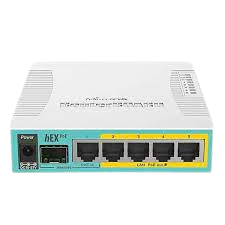
\includegraphics[width=0.7\linewidth]{P3/img/contoh.png}
        \caption{Gambar Contoh}
        \label{fig:gambarcontoh}
    \end{figure}

    \subsection{Tugas Pendahuluan}
    \begin{enumerate}
        \item Halo
    \end{enumerate}


    \begin{center}
        \colorbox{cyan!30}{\parbox{0.8\linewidth}{\textbf{Opsional:} Pelajari Git dan Github. Anda dapat memulai pembelajaran dari sumber berikut ini: \\ \href{https://github.com}{GitHub - https://github.com} \\ \href{https://git-scm.com/doc}{Git -https://git-scm.com/doc}}}
    \end{center}
\end{comment}
\section{Pendahuluan}
\subsection{Latar Belakang}
Manajemen bandwidth adalah suatu pendekatan yang digunakan untuk mengatur dan
mengontrol penggunaan bandwidth dalam suatu jaringan komputer. Dalam jaringan yang
sibuk, alokasi bandwidth yang efisien dan adil sangat penting untuk menjaga kinerja jaringan
yang optimal. Salah satu cara untuk mengimplementasikan manajemen bandwidth adalah
dengan menggunakan QoS atau Quality of Service.